\chapter{Spectrometer Alignment} \label{ch::alignment}

The alignment of the spectrometer is important for track reconstruction.
Alignment is a part of pre-processing which ensures all the tracking detectors
are centered relative to each other and therefore enables the track resolution
to be as accurate as possible.  Without accurate alignment track reconstruction
is not possible and it is therefore not possible to analyze any data.  The
author of this thesis spent the summer of 2015 collecting alignment data and was
responsible for performing the alignment of the COMPASS spectrometer in 2015.

The objective of the alignment procedure is to produce a file called the
detectors.dat.  This file describes the parameters for all detectors at COMPASS
and in particular, gives their relative orientation from each other.  For a
tracking detector plane, there are four parameters the alignment procedure
updates: the x central position, y central position, angle and the pitch.  These
parameters are described in the COMPASS lab frame and the pitch refers to a
sense wire distance for wire chambers or central strip distance for detectors
with strip readouts.  One or two detectors.dat files was produced for each data
taking period.  The goal of the alignment procedure is to have all four
parameters aligned relative to each other for each tracking plane.

The alignment procedure works by minimizing the distance between all the
detector plane hit positions and a track position.  This task is difficult
because there are over 300 detectors planes described in the detectors.dat.  To
accomplish this minimization, a large amount of quality data is needed and
several specific matrix manipulations are utilized in the minimization
procedure~\cite{matrix_inv}.  This chapters gives an overview of the alignment
procedure and some results from 2015, for a more complete review see
reference~\cite{compassAlignmentNote}.


\section{Alignment Data}

The alignment data comes from dedicated low intensity muon beam, $\approx 10^5
\frac{\mu ^-}{\mathrm{spill}}$, data.  A muon beam is desirable for alignment
data because the beam muons interact less and therefore allow the alignment
procedure to assume straight tracks in the minimization problem.  The lower
intensity is chosen because this allows the assumption that only one track
occurs per event and a low intensity beam ensures a reduction of detector pile
up effects.  Reduction in pile up effects, makes reconstruction in the central
detector areas possible, and therefore the beam killers on DC00, DC01, DC04 and
DC05 can be set to nominal voltage and as well all the GEM detectors can
have their central high voltages turn up to an amplification voltage.

A dedicated trigger system is setup during alignment runs to maximize the
illumination of the tracking detectors.  The triggers used are a beam trigger,
veto trigger and a halo trigger.  The alignment runs used in 2015 are listed in
Table~\ref{tab::alignmentRuns}. \par

Two good quality alignment runs are recorded either at the beginning, middle or
end of a data taking period.  The first alignment run is with the spectrometer
magnets off and the second is with the spectrometer magnets on.  The
spectrometer magnets off run is used as a first iteration for the alignment
procedure to initialize the tracking detector positions.  The final alignment
positions are then determined from the spectrometer magnets on data.

In 2015 the alignment runs were performed when the target solenoid was
polarizing the target.  The chicane magnets upstream of the target were
therefore turned off to ensure the beam momentum was traveling along the target
axis.  Normally to achieve the reduced intensity, the T6 target is switch to an
air target, however in 2015 the T6 target head was not able to switch between
the different target lengths and therefore the maximum 500~mm target head was
always in use.  Therefore to achieve the desired intensity, a set of collimeters
upstream of the target reduced the aperture of the beam line till the correct
intensity was achieved.

\begin{table}[h!t]
  \centering
  \begin{tabular}{ |c|c|c|c|c|c| }
    \hline
    \textbf{Period}& \textbf{Sub-period}& \textbf{Magnets off run}&
    \textbf{Magnets on run}& \textbf{Physics run}&
    \textbf{detectors.dat name} \\ \hline
    
    W07& one \& two & 259360& 259361& 259363& detectors.259361.transv.dat
    \\ \hline

    W08& one \& two & 260072& 260073& 260100& detectors.260073.transv.dat
    \\ \hline

    \multirow{2}{2em}{W09}& one& 260625& 260626& 260661&
    detectors.260626.transv.dat \\
    & two& 260625& 260876& 261312&
    detectors.260876.transv.dat \\ \hline

    \multirow{2}{2em}{W10}& one& 261512& 261513& 261602&
    detectors.261513.transv.dat \\
    & two& 261512& 261513& 261974&
    detectors.261970.transv.dat \\ \hline

    W11& one \& two & 262423& 262425& 262612& detectors.262370.transv.dat
    \\ \hline

    W12& one \& two & 263139& 263140& 263175& detectors.263140.transv.dat
    \\ \hline

    W13& one \& two & 263636& 263637& 263851& detectors.263637.transv.dat
    \\ \hline

    W14& one \& two & none& 264428& 264429& detectors.264163.transv.dat
    \\ \hline

    W15& one \& two & 264614& 264722& 264736& detectors.264619.transv.dat
    \\ \hline
    
  \end{tabular}
  \caption{COMPASS 2015 alignment data runs}
  \label{tab::alignmentRuns}
\end{table}


\section{Procedure}

The starting point for alignment is a detectors.dat file with tracking detector
positions determined from a survey.  The surveys are performed with the
spectrometer magnets off and the precision from a survey is around 1~mm.  Almost
all of the detectors at COMPASS have a position resolution better than the
survey precision.  Furthermore, several detectors near SM1 can shift in position
due to the magnetic field and therefore need a position determination with the
spectrometer magnets on.  For these reasons the alignment procedure is needed to
improve on the survey precision and achieve the best possible track resolutions.

\subsubsection{Alignment Parameters}

To best describe each detector relative to every other detector there are two
reference systems of interest.

The first is the COMPASS main reference system labeled \textit{Oxyz}.  This
reference system can also be referred to as the COMPASS lab system, where the
z-axis is along the beam momentum direction, the y-axis points vertical and the
x-axis is such that the coordinate system is right handed.  The origin of this
reference system is at the center of the target from the original COMPASS setup.

The second reference system is the local reference system, which is labeled as
\textit{O'uvz}.  This reference system is different for each detector and has
its origin at the center of each detector center.  The z-axis coincides with the
z-axis in the COMPASS main reference system while the u-axis is in the direction
along the measure coordinate of the detector, and the v-axis is perpendicular to
the direction of the measure coordinate of the detector.  As an example, a drift
chamber with vertical wires measures a coordinate along the horizontal direction
and therefore it's u-axis is in the horizontal direction and it's v-axis is in
the vertical direction.  A drift chamber with horizontal wires, however,
measures a coordinate along the vertical direction and therefore it's u-axis is
in the vertical direction and it's v-axis is in the horizontal direction.

The alignment parameters are defined in \textit{O'uvz}.  The alignment procedure
updates the starting detectors.dat file by the shifts

\begin{align}
  \delta \mathrm{u} & \mathrm{: \; shift \; in \; u \; direction,}  \\
  \delta \theta & \mathrm{: \; shift \; in \; rotation \; angle,}  \\
  \delta \textrm{z} & \mathrm{: \; shift \; in \; z \; direction,}  \\
  \delta \textrm{p} & \mathrm{: \; shift \; in \; pitch.} 
\end{align}
\noindent
The shift in z direction has never converged however.  As a result the z
coordinate from the survey is used as the final z position and the shift in
pitch is used as an effect shift in the z direction.

\subsubsection{Minimization}

The goal of the alignment procedure is to minimize the distance of a track
positions through a detector with respect to where the detector measures the
track position.  Due to the fact that the alignment tracks are assumed to be
straight, each track can be defined by four parameters.  The track parameters,
{\atrack}, are

\begin{enumerate}[label=\roman*:]
\item (x, y) the x and y coordinates at the main reference origin
\item (t$_{\mathrm{x}}$, t$_{\mathrm{y}}$) the tangents of the track momentum in
  the x and y directions at the origin of the main reference system
\end{enumerate}
\noindent
where the track parameters are defined for each track.  The alignment parameters
, {\adet}, on the other hand are defined for each detector but are the same for
all tracks.  The alignment procedure minimizes the $\chi^2$ function

\begin{equation}
  \chi^2 = \sum_{i=1}^{i=n_{\mathrm{tracks}}}\sum_{j=1}^{j=n_{\mathrm{detectors}}}
  \frac{\mathrm{F}^2_j(\alpha_{\mathrm{T}, i}, \alpha_{\alpha, j})}{\sigma_j^2},
  \label{equ:chi_align}%
\end{equation}
\noindent
where $\sigma^2_j$ is the position resolution of detector j.  The function F is
the residual distance of each detector which is the distance between where a
detector measures a track position and the track position.

\section{Results}
  The alignment procedure accomplishes this by minimizing a
$\chi^2$ function of all the track and detector parameters:
%
%\begin{dmath}
%  \chi^2 = \sum_{i=1}^{i=n_{tracks}}\sum_{j=1}^{j=n_{detectors}}
%  \frac{F_j(\alpha_t, \alpha_j)^2}{\sigma_j^2},
%  \label{equ:chi_align}%
%\end{dmath}
%
where $F_j(\alpha_t, \alpha_j)$ is the residual of each detector plane
and is a function of the track parameters, $\alpha_t$, and the
detector parameters, $\alpha_j$, and $\sigma_j$ is the position
resolution for detector $j$. The residual, $F_j(\alpha_t, \alpha_j)$,
is the difference between a detector hit location and the expexted hit
location based on a reconstructed track.  The track parameters,
$\alpha_t$, are the track x and y position at a specified detector and
the tangents $\frac{dx}{dz}$ and $\frac{dy}{dz}$ of the track momentum
at the same location.  These track parameters are different for each
track while the detector parameters, $\alpha_j$,
are the same for every track.  \par





To perform the $\chi^2$ minimization in the alignment procedure,
$F_j(\alpha_t, \alpha_d)$ is Taylor expanded and the partial
derivative of the $\chi^2$ function, equation~\ref{equ:chi_align}, is
taken with the respect to each track and alignment parameter and set
equal to zero.  The minimization process can be built into a matrix
equation where the size of the matrix to invert is
$(4n_{detector}+4n_{tracks})\times(4n_{detector}+4n_{tracks})$: \par
%
\begin{subequations}
  \begin{align}
    &F_j = F_j^0 + \sum_k \frac{\partial F_j}{\partial
      \alpha_k}\alpha_k \quad \text{Taylor expanding the residual for
      each detector plane.} \label{equ:F_taylor}\\ &\frac{1}{2}
    \frac{\partial \chi ^2}{\partial \alpha_i} = \sum
    _{t}^{n_{tracks}} \sum_j ^{n_{detectors}}\frac{1}{\sigma_j
      ^2}\frac{\partial F_j}{\partial \alpha_i}\Big ( F_j^0 + \sum_k
    \frac{\partial F_j}{\partial \alpha_k}\alpha_k \Big ) = 0 \quad
    \text{Minimizing the overall $\chi^2$.}\\ & \begin{bmatrix} \sum_j
      \frac{1}{\sigma^2_j}\frac{\partial F_j}{\partial
        \alpha_1}\frac{\partial F_j}{\partial \alpha_1} & \dots &
      \sum_j \frac{1}{\sigma^2_j}\frac{\partial F_j}{\partial
        \alpha_1}\frac{\partial F_j}{\partial \alpha_{4n_{tracks}}}
      \\ \vdots & \ddots & \vdots\\ \sum_j
      \frac{1}{\sigma^2_j}\frac{\partial F_j}{\partial
        \alpha_{4n_{tracks}}}\frac{\partial F_j}{\partial \alpha_1} &
      \dots & \sum_j \frac{1}{\sigma^2_j}\frac{\partial F_j}{\partial
        \alpha_{4n_{tracks}}}\frac{\partial F_j}{\partial
        \alpha_{4n_{tracks}}}
      \end{bmatrix}
    \begin{bmatrix}
      \alpha_1 \\ \vdots \\ \alpha_{4n_{tracks}}
    \end{bmatrix}
    = -
    \begin{bmatrix}
      \sum_j \frac{1}{\sigma^2_j}\frac{\partial F_j}{\partial
        \alpha_1} F_j^0 \\ \vdots \\ \sum_j
      \frac{1}{\sigma^2_j}\frac{\partial F_j}{\partial
        \alpha_{4n_{tracks}}} F_j^0 \\
    \end{bmatrix} \label{equ:aliMatrix}
  \end{align}
  \label{equ:Alignment}
\end{subequations}
%    %\text{Resulting equation to be solved.}
A normal alignment run results in over 200,000 tracks meaning the
matrix equation in equation~\ref{equ:aliMatrix} is huge and infeasible
to solve.  Fortunately many of the entries in the matrix are zero and
it can be shown that this matrix inversion can be reduced to the
inversion of several smaller matrices~\cite{matrix_inv}.  \par

%\begin{figure}[h]
%  \centering
%  \begin{subfigure}[t]{0.3\textwidth}
%    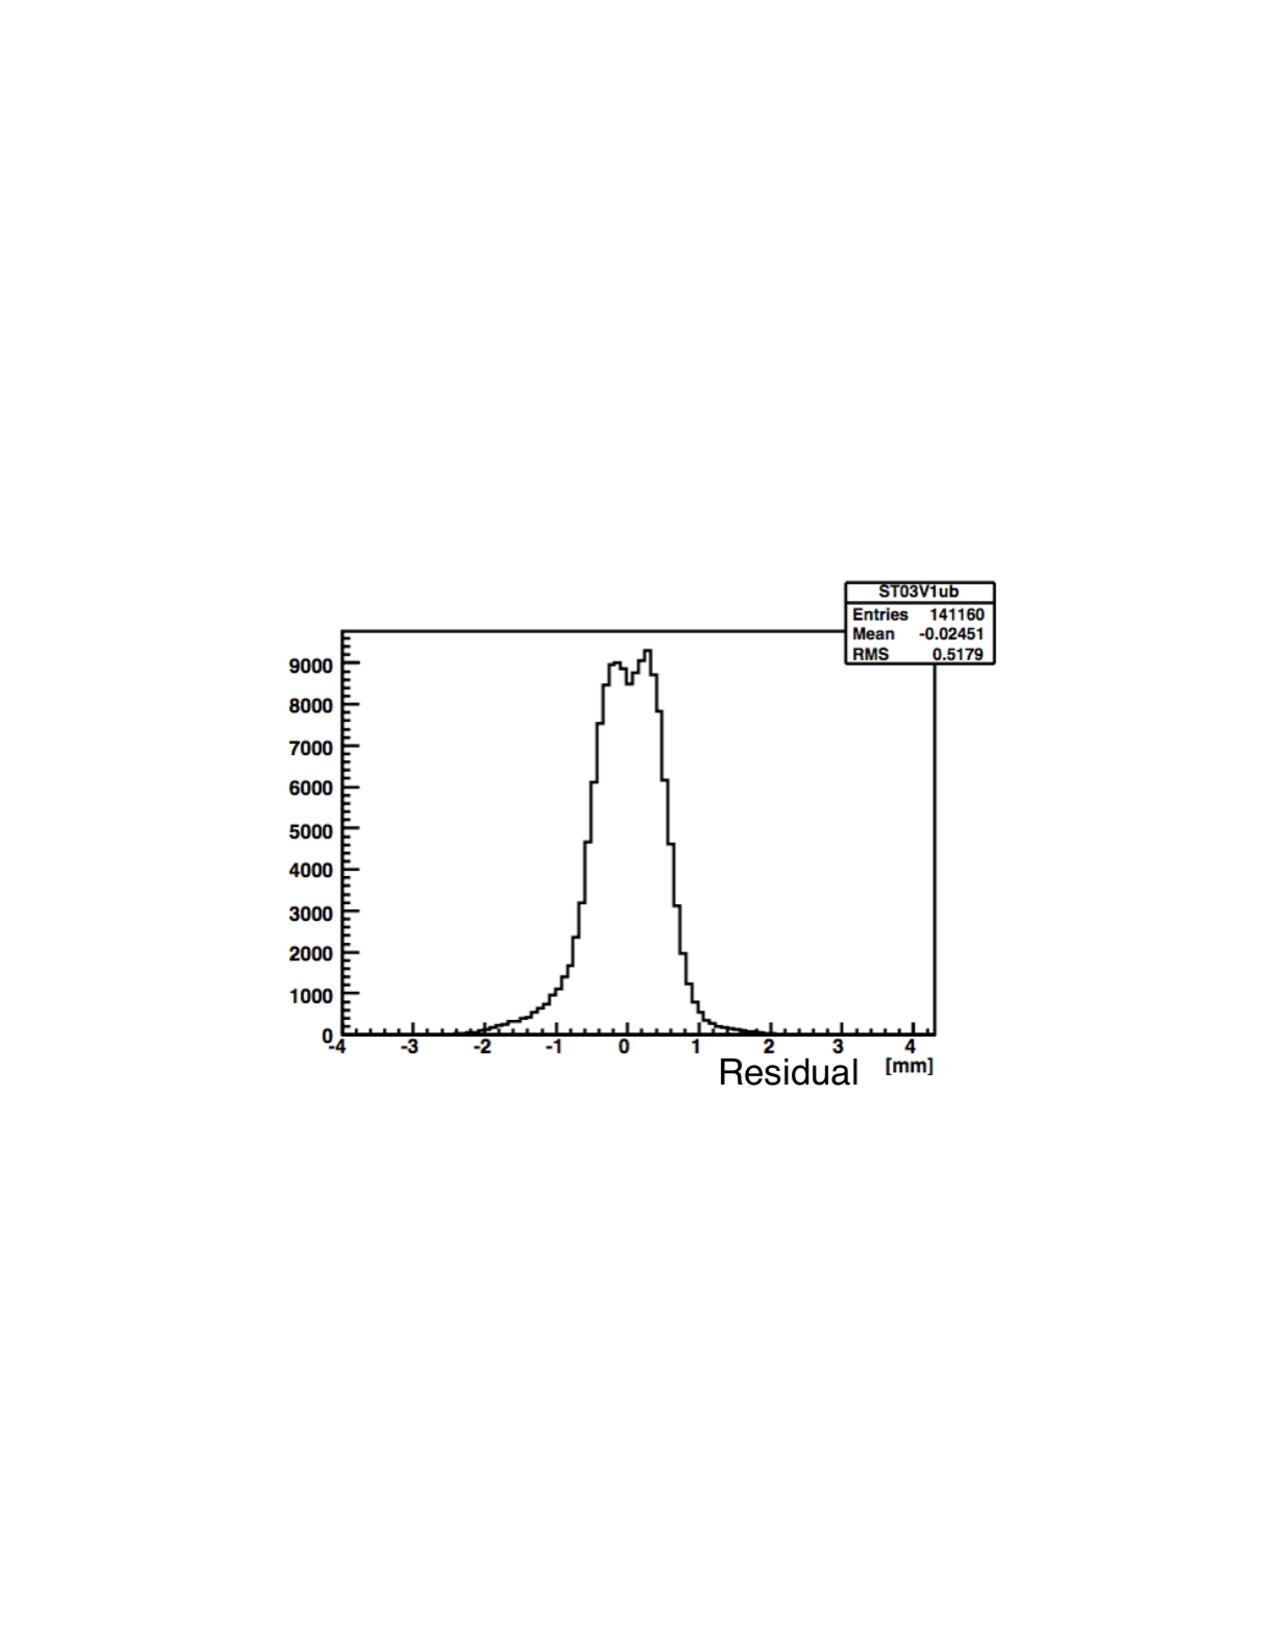
\includegraphics[width=\textwidth]{PositionResidual}
%    \caption{This plot tells if the detector is shifted in position or
%      not.}
%    \label{fig:PosRes}%
%  \end{subfigure}
%  \begin{subfigure}[t]{0.3\textwidth}
%    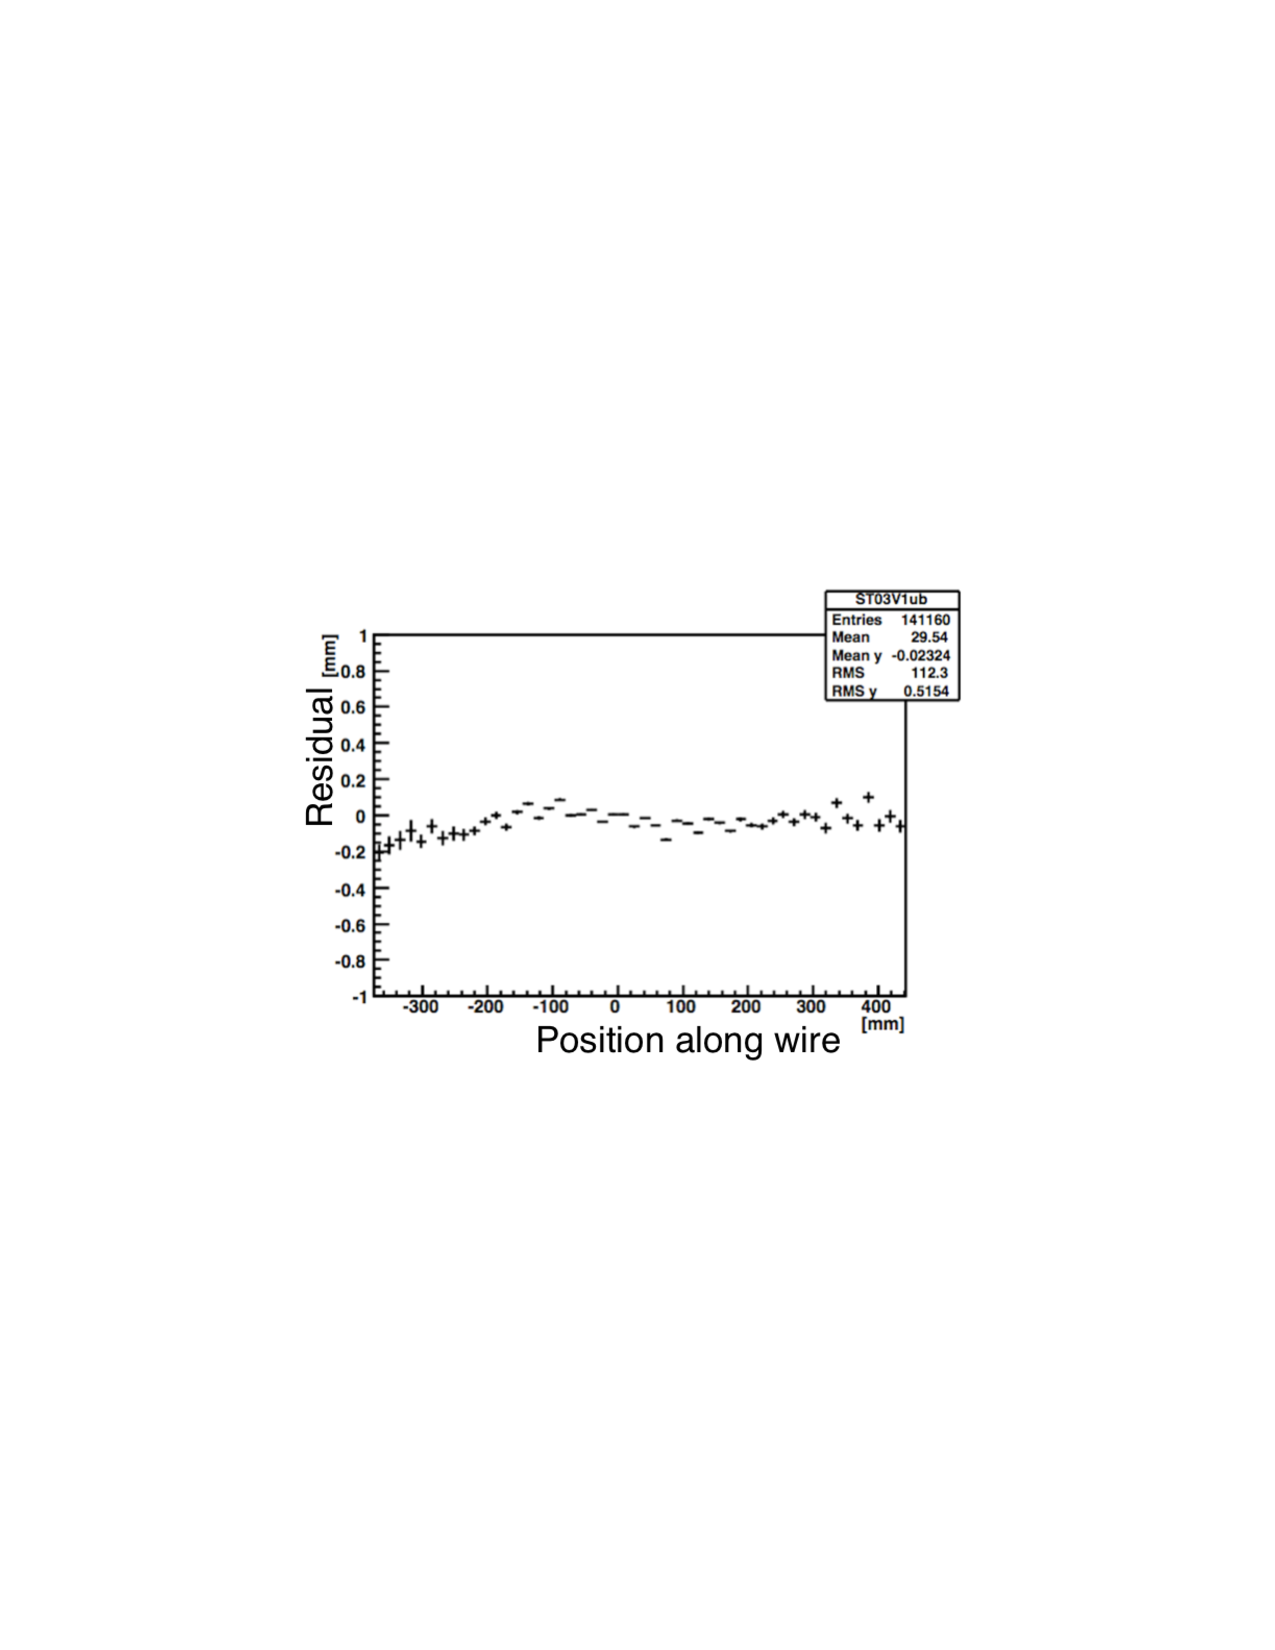
\includegraphics[width=\textwidth]{AngleResidual}
%    \caption{This plot is used to determine if the detector has the
%      correct angle.}
%    \label{fig:AngRes}%
%  \end{subfigure}
%  \begin{subfigure}[t]{0.3\textwidth}
%    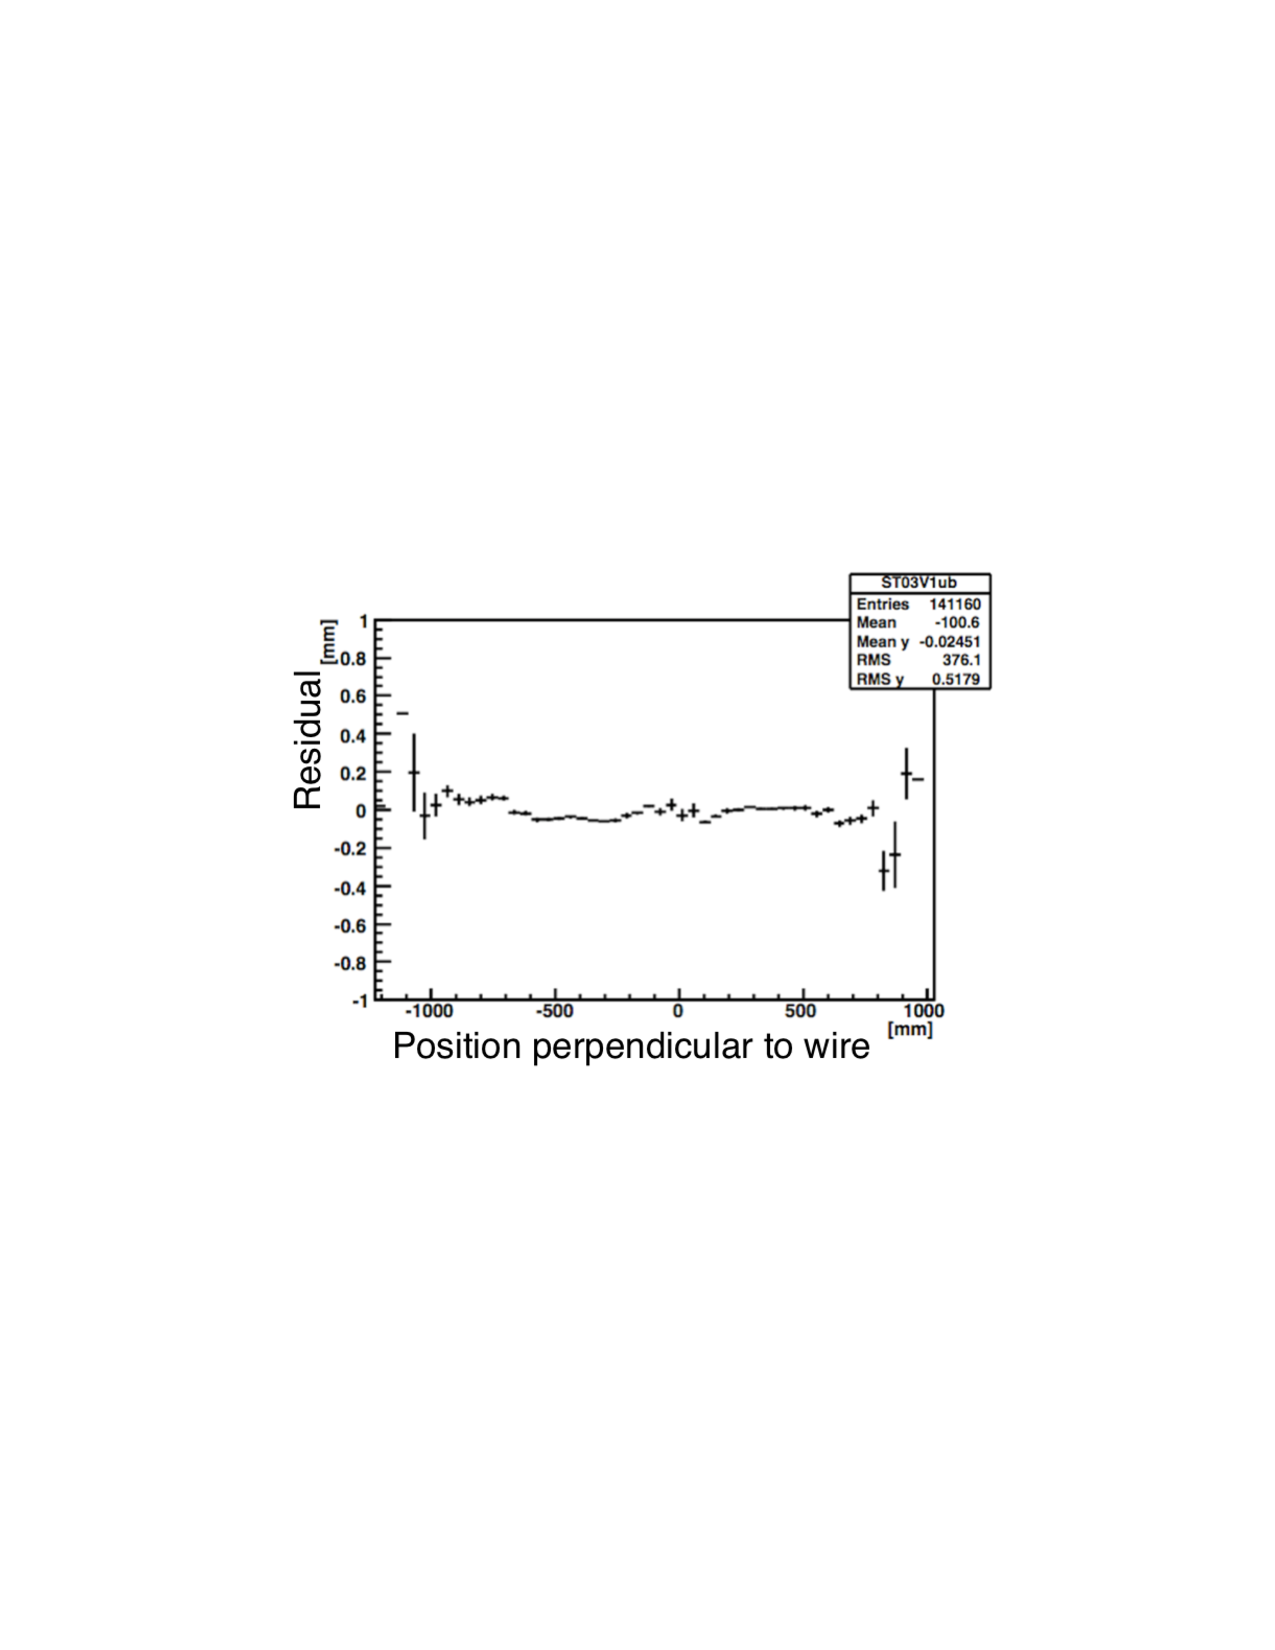
\includegraphics[width=\textwidth]{PitchResidual} 
%    \caption{This plot is used to determine if the detector wires have
%      the correct pitch.}
%    \label{fig:PitchRes}%
%  \end{subfigure}
%  \caption{Different residual distributions for a plane of a straw
%    detector at COMPASS.}
%  \label{fig:AlignRes}
%\end{figure}

In each iteration of the alignment procedure the matrix inversion in
equation~\ref{equ:aliMatrix} is performed.  All alignment tracks are
reconstructed based off the starting positions of all the detectors
and after each iteration the detector parameters are updated to reduce
the overall $\chi^2$ value.  Several iterations of the alignment
procedure are therefore required and are performed to ensure the
procedure converges.\par

The final product of the alignment procedure is an alignment file, for
each data period, that describes the location of every detector and is
used in all the data analysis.  For quality assurance several residual
distributions are plotted after each iteration for all the detectors.
The overall residual distribution is used to tell if a detector is
shifted, the change in residual as a function of the distance parallel
to the wires tells if a detector is rotated and the change in residual
as a function of the distance perpendicular to the wires tells if a
detector has been assigned the correct wire pitch in the alignment
file.  Examples of these residuals, to check are shown in
figure~\ref{fig:AlignRes}.


